\begin{flushright}
    \textit{Лекция 1 (от 07.09)}
\end{flushright}
\section{$\S 1.$ Комплексные числа}
\Def
Пусть $z = \left( x;y \right) \in \RR^2$. Пусть определены операции:
\begin{enumerate}
    \item \textbf{Сложение:} $z_1 + z_2 = \left( x_1+x_2; y_1+y_2 \right)$
    \item \textbf{Умножение на действительное число:} $\lambda z = \left(\lambda
        x, \lambda y \right)$
    \item \textbf{Расстояние:} $\rho(z_1, z_2) = \left| \left| z_1 - z_2 \right|
    \right| = \sqrt{\left( x_1 - x_2 \right)^2 + (y_1 - y_2)^2}$
\end{enumerate}
Добавим операцию
умножения друг на друга:
\begin{align*}
  & z_1 \cdot z_2 = \left( x_1 \cdot x_2 - y_1 \cdot y_2; x_1 \cdot y_2 + x_2 \cdot y_1 \right)
\end{align*}
Будем называть это \textbf{комплексными числами} $\CC$.
\\
Пусть $1 \sim (1; 0)$~--- \textbf{единица}, $i \sim (0;1)$~--- \textbf{мнимая
  единица}.
\\
Тогда $z = 1 \cdot x + i \cdot y \Leftrightarrow z = x + iy$~---
\textbf{алгебраическая запись}.
\\
Назовем $x = \Real z$ \textbf{действительной частью}, $y =
\Img z$~--- \textbf{мнимой}.
\\
\textbf{Сопряженным} к $z = x+iy$ называем $\bar{z} = x-iy$,
\textbf{модулем}~--- выражение $\left| z \right| = \sqrt{x^2+y^2}$. Легко
видеть, что $z\bar{z} = \left| z \right|^2$, полагая $i^2 = -1$.
\\
Можно представлять комплексные числа в виде $x = r \cos \varphi$, $y = r \sin
\varphi$, называя $r$ \textbf{модулем}, $\varphi$ \textbf{аргументом}, а $\arg z
\in (-\pi; \pi]$~--- одно из таких $\varphi$~--- \textbf{главным аргументом}.
Также \textbf{аргументом} называется множество $\Arg z = \left\{ \arg z + 2\pi k
    \mid k \in \ZZ \right\}$.
\\
Видим, что
\begin{align*}
  & z = \left| z \right|\cos \varphi + i \left| z \right|\sin \varphi = \left| z \right|\left( \cos \varphi + i \sin \varphi \right)
\end{align*}
Введем \textbf{комплексную экспоненту}~--- $e^{i\varphi} = \cos \varphi + i \sin
\varphi$, тогда $z = \left| z \right|e^{i\varphi}$.
\\
Для произведения тогда выполняется
\begin{align*}
  & z_1z_2 = \left| z_1 \right|\left( \cos \varphi_1 + i \sin \varphi_2 \right)\left| z_2 \right|\left( \cos \varphi_2 + i \sin \varphi_2 \right) = \left| z_1 \right|\cdot \left| z_2 \right| \left( \cos \left( \varphi_1+\varphi_2 \right) + i \sin \left( \varphi_1+\varphi_2 \right)\right)
\end{align*}
\begin{align*}
  & \left|z_1z_2\right| = \left| z_1 \right|\cdot \left| z_2 \right|
\end{align*}
\begin{align*}
  & \Arg(z_1z_2) = \Arg z_1 + \Arg z_2
\end{align*}
\textbf{Суммой Минковского} называется множество $A+B = \sets{a+b \mid a\in A, \
  b \in B}$.
\\
На комплексных числах определено \textbf{деление} на $z\neq 0$: $z_1z = z_2
\Rightarrow z = \dst \frac{z_2}{z_1}$; если $z_2=1$, то $z = \dst \frac{1}{z_1}
= z_1^{-1}$.
\\
Нахождение частного эквивалентно решению системы
\begin{align*}
  & \left\{ \begin{matrix}
          x_1x-y_1y=x_2 \\
          y_1x+x_1y = y_2
      \end{matrix} \right.
\end{align*}
Это можно выразить как
\begin{align*}
  & z = \frac{\bar{z_1}z_2}{\left| z_1 \right|^2} = \frac{\left| z_2 \right|e^{i \varphi_2}}{\left| z_1 \right| e^{i \varphi_1}} = \frac{\left| z_2 \right|}{\left| z_1 \right|}e^{i\left( \varphi_2-\varphi_1 \right)}
\end{align*}
Зная, что $e^{i \varphi_1}e^{i \varphi_2} = e^{i\left( \varphi_1+\varphi_2
  \right)}$, можем записать \textbf{формулу Муавра}:
\begin{align*}
  & \forall n \in \NN \ z^n = \left| z \right|^ne^{i n \varphi} 
\end{align*}
Также определена операция \textbf{извлечения корня} из $z^n = a \neq 0$.
Полагаем $z=re^{i\varphi}$, $a = \left| a \right|e^{i\alpha}$. Тогда $r^n =
\left| \alpha \right|$, а $n \varphi = \alpha + 2 \pi k, \ k \in \ZZ$. Отсюда $r
= \sqrt[n]{\left| a \right|}$, $\varphi_k = \dst \frac{\alpha+2\pi k}{n}$. тогда
определим корень как
\begin{align*}
  & \sets{\sqrt[n]{a}} = \sets{\sqrt[n]{\left| a \right|}\left( \cos \frac{\alpha + 2 \pi k}{n} + i \sin \frac{\alpha + 2 \pi k}{n} \right)\mid k \in \{0, \dots, n-1\}}
\end{align*}
\Example
\begin{align*}
  & \sets{\sqrt[4]{i}} = \sets{\exp\left( i \frac{\dst \frac{\pi}{2} + 2 \pi k}{4} \right)\mid k \in \{0, \dots, 3\}}
\end{align*}
\section{$\S 2.$ Последовательность. Предел. Ряды. Функции. Расширенная
  комплексная плоскость}
\Def
\textbf{Окрестностью} назовем $B_r(z_0) = \left\{ z \in \CC: \left| z-z_0
    \right| < r \right\}$. \textbf{Проколотой окрестностью} назовем $B_r(z_0) =
\left\{ z \in \CC: 0 < \left| z-z_0 \right| < r \right\}$. \textbf{Замкнутой
  окрестностью} назовем $B_r(z_0) = \left\{ z \in \CC: \left| z-z_0\right| \leq
    r \right\}$.
\Def
Множество $\left\{ z_n \right\}_{n=1}^\infty$, $z_n  = x_n + iy_n$ называется
\textbf{последовательностью}.
\Def
Число $A \in \CC$ называется \textbf{пределом последовательности $z_n$} (пишем
$\dst \lim_{n \to \infty}z_n = A$) тогда и только тогда, когда выполняется
\begin{equation}\label{(2.1)}
    \forall \varepsilon > 0 \exists N(\varepsilon):\forall n \geq N(\varepsilon)\in \NN \hookrightarrow z_n \in B_{\varepsilon}(A)
\end{equation}
\asm
\begin{align*}
  & \exists \lim_{n \to \infty}z_n = A = a+ib \Leftrightarrow \left\{ \begin{matrix}
          \dst \lim_{n \to \infty}x_n = a \\
          \dst \lim_{n \to \infty}y_n = b
      \end{matrix} \right.
\end{align*}
\pr Докажем в обе стороны.
\begin{itemize}
    \item $\Rightarrow$:
    \begin{align*}
      & \left| x_n - a \right| \leq \left| z_n - A \right| < \varepsilon
    \end{align*}
    \begin{align*}
      & \left| x_n - a \right| \leq \left| z_n - A \right| < \varepsilon
    \end{align*}
    \item $\Rightarrow$:
    \begin{align*}
      & \exists N_z(\varepsilon) = \max\left\{ N_x\left( \frac{\varepsilon}{2} \right), N_y\left( \frac{\varepsilon}{2} \right) \right\}: \forall n \geq N_z(\varepsilon) \hookrightarrow \\
      & \left| z_n-A \right|\leq \left| x_n-a \right|+\left| y_n-b \right| < \frac{\varepsilon}{2} +\frac{\varepsilon}{2} = \varepsilon
    \end{align*}
\end{itemize}
\corollary
Все свойства последовательностей действительных чисел (пределы суммы,
произведения, критерий Коши и т.~д.) переносятся на последовательности
комплексных.
\Def
\textbf{Рядом, порожденным последовательностью $\left\{ z_n \right\}$}, называют
последовательность $S_N = \dst \sum_{n=1}^Nz_n$. Говорят, что ряд
\textbf{сходится}, если $\dst \lim_{N \to \infty}S_N = S$. Этот предел называют
\textbf{суммой ряда} и записывают как $\dst \sum_{n=1}^\infty z_n$.
\asm
Сходимость $\dst \sum_{n=1}^\infty z_n$ равносильна сходимости $\dst
\sum_{n=1}^\infty x_n$ и $\sum_{n=1}^\infty y_n$.
\pr
Очевидно из свойств пределов и критерия Коши.
\Def
Говорят, что $\dst \lim_{n\to \infty}z_n = \infty$, если $\forall \varepsilon >
0 \exists N(\varepsilon): \forall n \geq N(\varepsilon)\in \NN \hookrightarrow
\left| z_n \right|> \varepsilon$. \textbf{Окрестностью бесконечности} называют
$B_\varepsilon(\infty) = \left\{ z \in \CC: \left| z \right| > \varepsilon
\right\}$.
\Def
\textbf{Расширенной комплексной плоскостью} $\CCC$ называается $\CC \cup \left\{
    \infty \right\}$, причем $\infty$ вводится с системой окрестностей.
\Note
$\CCC$~--- компакт.
\pr ~
\begin{itemize}
    \item Если $\left\{ z_n \right\}$ ограничена, то по теореме Вейерштрасса
    можно выделить подпоследовательность, сходящуюся к $z \in \CC$.
    \item Если $\left\{ z_n \right\}$ неограничена, то $\forall k \in \NN
    \exists n_k > n_{k-1}: \ \left| z_{n_k} \right| > k$, а занчит, $z_n \to
    \infty \in \CCC$.
\end{itemize}
Значит, это компакт.
\\
Рассмотрим $\RR^3$ с координатами $(\xi, \eta, \zeta)$. Пусть $\xi = x$, $\eta =
y$, $z = x+iy \in \CC$.
\Def
\textbf{Сфера Римана:}
\begin{equation}\label{(2.2)}
    S: \ \xi^2+\eta^2+\zeta^2 = \zeta
\end{equation}
\begin{figure}[h!]
		\centering
		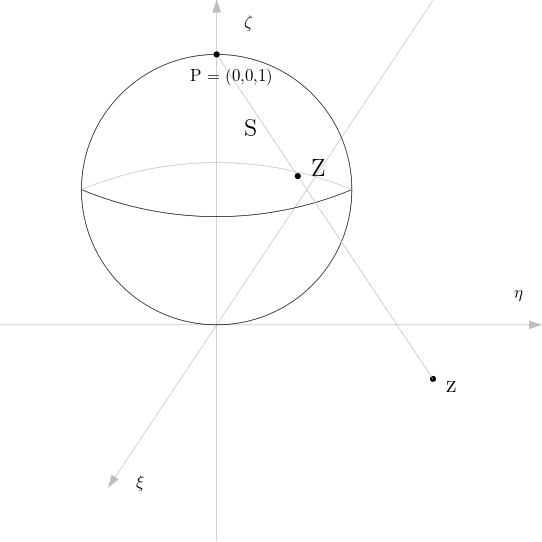
\includegraphics[scale=0.5]{Riemann.png}
    \caption{Сфера Римана}
		\label{fig:2.1}
\end{figure}
\Def
\textbf{Стереографическая проекция:}
\begin{align*}
  & \forall z \in \CC \exists Z \in (\xi, \eta, \zeta): \ \left\{ \begin{matrix}
          \xi = tx \\
          \eta = ty \\
          \zeta = 1-t
      \end{matrix} \right., \ t \in [0;1]
\end{align*}
\begin{align*}
  & t = \frac{1}{1+ \left| z \right|^2}, \ \xi = \frac{x}{1+ \left| z \right|^2}, \ \eta = \frac{y}{1+ \left| z \right|^2}, \ \zeta = \frac{\left| z \right|^2}{1+ \left| z \right|^2}
\end{align*}
\begin{align*}
  & S \setminus P \leftrightarrow \CC, \ P \leftrightarrow \infty
\end{align*}
\textbf{Свойства}
\begin{enumerate}
    \item Любая пряая или окружность на комплексной плоскости переходит в
    окружность на сфере Римана.
    \item Если любые две кусочно гладкие кривые $\gamma_1$ и $\gamma_2$
    пересекаются под углом $\alpha$ на комплексной плоскости, то их образы
    $\tilde{\gamma}_1$, $\tilde{\gamma}_2$ будут пересекаться под тем же углом
    $\alpha$ на сфере Римана.
\end{enumerate}
\Def
$f: G \mapsto D$, где $G$~--- область, $D \subseteq \CCC$~--- область или вся
(расширенная) комплексная плоскость; $f(z) = u(x,y) + iv(x,y)$~---
\textbf{функция комплексного переменного.}
\Def
Пусть $z_0$~--- предельная точка $G \subseteq \CCC$ и $f: G \mapsto \CCC$; тогда
число $A$ назыается \textbf{пределом} $f$ в этой точке (пишется $\dst \lim_{z \to
  z_0} f(z_0)$) тогда и только тогда, когда выполняется
\begin{equation}\label{(2.3)}
    \forall \varepsilon > 0 \exists \delta(\varepsilon) > 0: \ z \in \os{\circ}{B}_\delta(z_0)\cap G \hookrightarrow f(z) \in B_\varepsilon (A)
\end{equation}
\asm
\begin{align*}
  & \exists \lim_{z \to z_0}f(z) = A = a+ib \Leftrightarrow \left\{ \begin{matrix}
          \dst \lim_{(x,y)\os{G}{\to}(x_0,y_0)}u(x,y) = a \\
          \dst \lim_{(x,y)\os{G}{\to}(x_0,y_0)}v(x,y) = b
      \end{matrix} \right.
\end{align*}
\pr
Очевидно по аналогии с последовательностями.
\Def
$f: G \mapsto \CCC$ \textbf{непрерывна} в $z_0 \in G \subseteq \CCC$, если
$z_0$~--- предельная точка $G$ и $\dst \lim_{z \to z_0} = f(z_0)$.
\asm
Функция непрерывна тогда и только тогда, кода ее действителная и мнимая части
непрерывны.
\pr Очевидно по аналогии с пределом.
\Def
\textbf{Функциональным рядом} называется сумма вида $\dst \sum_{n=1}^\infty
f_n(z)$, где $\forall n \in \NN \ f_n :G \mapsto \CC$.
\Def
Ряд \textbf{сходится равномерно}, если он:
\begin{enumerate}
    \item $\forall z \in G$ сходится к некоторой $S(z)$;
    \item $\forall \varepsilon > 0 \exists N(\varepsilon) > 0: \forall N \geq N
    (\varepsilon) \ \left| \dst \sum_{n=1}^Nf_n(z) - S(z) \right|\leq
    \varepsilon$.
\end{enumerate}
Все критерии и признаки для таких рядов аналогичны таковым в действительном
анализе.    